% \renewcommand{\labelitemi}{$\blacktriangleright$}
% \renewcommand{\labelitemi}{$\triangleright$}
 \renewcommand{\labelitemi}{$\rhd$}
% \renewcommand{\labelitemi}{$\centerdot$}

~\newline
%===============================================================================
\chapter{Supercooling and suspended frazil ice}
\label{chapter:tracers}
%===============================================================================

%---------------------------------------------------------------------------
\section{Suspended Frazil Ice}

In nature the frazil ice crystal distribution is non-homogeneous and often follows a log-normal distribution
as observed in \cite{clark_2006} and \cite{macfarlane_2017}. Additionally the radius of each crystal is function of time
and depends on the thermal exchanges between the particle and the surrounding water.
This process, also known as the thermal growth (or decay), is a key aspect to describe the evolution frazil ice
evolution in water bodies.
There are two models available in \khione to describe frazil ice evolution, the SSC\footnote{SSC : single-size-class} model
and the MSC\footnote{MSC : multiple-size-class} model, which rely on different radius discretization as shown in Figure \ref{fig:radius_discretization}.

\begin{figure}[H]
    \begin{center}
        \includegraphicsmaybe{[width=0.78\textwidth]}{./graphics/ssc_vs_msc.png}
    \end{center}
    \caption{Typical log-normal distribution of frazil crystals and SSC (left) versus MSC (right) radius discretization.}
    \label{fig:radius_discretization}
\end{figure}

In the case of the SSC model, all particles are assumed to have the same radius, noted $r$.
Modelling thermal growth therefore consists in predicting the evolution of the global volume fraction of frazil without
describing the radius changes.
On the other hand, the MSC model consists in considering several classes, each one associated with a radius, noted $r_k$ for the $k^{\rm{th}}$ class.
Thermal growth (or decay) is then modelled as mass exchanges between classes which also corresponds to particles increasing (or decreasing) in size.
The selection of the model depends on the number of classes selected with the keyword
\telkey{NUMBER OF CLASSES FOR SUSPENDED FRAZIL ICE} (default = 1). If only one class is selected, the SSC model is used,
otherwise the MSC model is selected.
Note that the number of classes should be sufficiently large for the model to converge in radial space.

\paragraph{SSC model}
The SSC model relies on one tracer to model frazil ice volume fraction.
The radius of frazil ice crystals is assumed to be constant and representative of the whole
distribution of particles in the suspension. The mass balance equation of frazil ice reads:

\begin{equation}
  \frac{\partial C}{\partial t} + \vec{u} . \nabla C = \dfrac{1}{h} \nabla . \left( h \nu_{t,C}  \nabla C \right) +  S_{GM} + S_{SR} + S_M,
\label{eq:model:frazil}
\end{equation}
in which,
\begin{itemize}
	\item $C$ is the frazil volume fraction,
	\item $\nu_{t,C}$ is diffusivity of frazil,
	\item $S_{GM}$ is the thermal growth (or melting) source term described in section \ref{section:thermal_growth},
	\item $S_{SR}$ is the seeding rate source term described in section \ref{section:seeding}, which can be activated using the keyword \telkey{MODEL FOR FRAZIL SEEDING} = 2 or 3 (default = 1).
  \item $S_M$ is the mass exchange source term (deposition/erosion under the ice cover) and can be activated with the keyword \telkey{MODEL FOR MASS EXCHANGE BETWEEN FRAZIL AND ICE COVER} (default = 0).
\end{itemize}

\paragraph{MSC model}
As opposed to the SSC model, the MSC model relies on
a discrete radius distribution to describe suspended frazil ice in which
a number of classes (noted $N_c$) are used to model the suspension.
The mass balance equation of the frazil volume fraction for the $k^{\rm{th}}$ class is given by
\begin{equation}
\frac{\partial C_{k}}{\partial t} + \vec{u} . \nabla C_{k} = \dfrac{1}{h}  \nabla . \left( h\nu_{t,k}  \nabla C_k \right) +  S_{GM}^{k} + S_{SN}^{k} + S_{FB}^{k} + S_{SR}^{k} + S_M^k,
\label{eq:model:frazil}
\end{equation}

\begin{itemize}
	\item $C_k$ is the frazil volume fraction of the $k^{\rm{th}}$ class,
	\item $\nu_{t,k}$ is diffusivity of frazil of the $k^{\rm{th}}$ class,
	\item $S^k_{GM}$ is the thermal growth (or melting) source term described in section \ref{section:thermal_growth},
	\item $S^k_{SN}$ is the secondary nucleation source term described in section \ref{section:secondary_nucleation}, which can be activated using the keyword \telkey{MODEL FOR THE SECONDARY NUCLEATION} (default = 2),
	\item $S^k_{FB}$ is the flocculation (and breaking) source term described in section \ref{section:flocculation}, which can be activated using the keyword \telkey{MODEL FOR THE FLOCCULATION AND BREAKUP} (default = 1),
	\item $S^k_{SR}$ is the seeding rate source term described in section \ref{section:seeding}, which can be activated using the keyword \telkey{MODEL FOR FRAZIL SEEDING} = 2 or 3 (default = 1).
  \item $S_M^k$ is the mass exchange source term by class (deposition/erosion under the ice cover) and can be activated with the keyword \telkey{MODEL FOR MASS EXCHANGE BETWEEN FRAZIL AND ICE COVER} (default = 0).
\end{itemize}
In this model, the total frazil volume fraction $C$ is computed as
\begin{equation}
C = \sum_{k=1}^{N_c} C_k.
\end{equation}
The number of particles per unit volume for each class is given by $n_k=C_k/V_k$ with $V_k$ the frazil crystal volume of class $k$.

\begin{WarningBlock}{Note:}
    The flocculation and secondary nucleation source terms are only computed in the MSC model
    i.e. if $N_c > 1$. If $N_c = 1$
    the keywords \telkey{MODEL FOR THE SECONDARY NUCLEATION} and \telkey{MODEL FOR THE FLOCCULATION AND BREAKUP}
    are automatically set to $0$.
\end{WarningBlock}

%---------------------------------------------------------------------------
\subsection{Shape of frazil crystals}
Frazil crystals are supposed to have the same disc shaped geometry, as described in Figure \ref{fig:crystal_shape}, characterized by a radius $r_k$ and a thickness $e_k$, related with a constant ratio $R$ such that $e_k = 2r_k/R$.
For the SSC description, the mean radius is defined via the keyword \telkey{FRAZIL CRYSTALS RADIUS} (default = 4.1E-4).
The thickness of each crytal is defined via the ratio $R$
which can be set with the keyword \telkey{FRAZIL CRYSTALS DIAMETER THICKNESS RATIO} (default = 10).

\begin{figure}[H]
    \begin{center}
        \includegraphicsmaybe{[width=0.35\textwidth]}{./graphics/crystal_shape.png}
    \end{center}
    \caption{Frazil crystal shape and parameters}
    \label{fig:crystal_shape}
\end{figure}

\begin{WarningBlock}{Note:}
 The number of radius provided must match the number of classes selected. For 3 classes, one could set:
 FRAZIL CRYSTALS RADIUS = 1.E-4 ; 2.E-4 ; 3.E-4
\end{WarningBlock}

%---------------------------------------------------------------------------
\subsection{Thermal growth and melting}
\label{section:thermal_growth}

Thermal growth or melting of frazil crystals depends on the heat exchange between the particle and the surounding water.
Let us first introduce the heat flux between frazil crystals of class $k$ and water in Equation \eqref{eq:model:sgm:heat_flux}:
\begin{equation}
q_k = \dfrac{K_w Nu_k}{l_k} (T_i - T),
\label{eq:model:sgm:heat_flux}
\end{equation}
where
\begin{itemize}
	\item $K_w$ is the thermal conductivity of water,
	\item $T_i$ the crystal temperature assumed to be equal to the freezing temperature $T_f$ which
is either defined with the keyword \telkey{FREEZING POINT OF WATER} (default = 0) or
depends on the salinity $S$ such that $T_f(S) = -0.0575S + 0.00171S^{3/2} - 0.00021S^2$ if \telkey{SALINITY=YES},
    \item $l_k$ is the characteristic length scale of the $k^{\rm{th}}$ class. It supposed to be equal to $e_k$ as suggested in \cite{jones_wells_2018},
    \item $Nu_k$ is the Nusselt number associated with the $k^{\rm{th}}$ class. Different methods can be selected to estimate the Nusselt number via the keyword \telkey{MODEL FOR THE NUSSELT NUMBER} (default=1).
\end{itemize}


\paragraph{MSC model}

The thermal growth (or decay) source term $S_{GM}^{k}$ represents the net rate of volume change of class $k$
resulting from interactions with classes $k-1$ and $k+1$ due to freezing or melting.
Following \cite{shen_JHR_2010} for thermal growth and \cite{holland_JFM_2005} for the introduction of melting, the net rate of volume fraction change for the frazil class $k$ can be defined as
\begin{equation}
S_{GM}^{k}=\frac{V_{k}}{\Delta V_{k-1}}\left [ (1-H)M_{k}+HG_{k-1} \right ]-\frac{V_{k}}{\Delta V_{k}}\left [ (1-H)M_{k+1}+HG_{k} \right ],
\label{eq:model:sgm:source}
\end{equation}
with
\begin{itemize}
	\item $H=He(T_{f}-T)$, where $He$ is the Heaviside function,
    \item $V_{k}$ the volume of ice crystals,
    \item $\Delta V_{k}$ the volume ratio defined by $\Delta V_{k}=V_{k+1}-V_{k}$ which accounts for the scaling of the computed volume change to the number of particles that jump from a class to another,
    \item $G_k$ and $M_k$ are the production or depletion rates of the $k^{\rm{th}}$ class, due to thermal growth or melting of frazil crystals.
\end{itemize}

Mass exchanges between classes (or class jumps) resulting from thermal growth or decay are explained in Figure \ref{fig:sgm_class_jumps}.
\begin{figure}[H]
    \begin{center}
        \includegraphicsmaybe{[width=0.45\textwidth]}{./graphics/sgm_class_jumps.png}
    \end{center}
    \caption{MSC model mass exchanges caused by thermal growth or melting}
    \label{fig:sgm_class_jumps}
\end{figure}

As explained in \cite{daly_1994}, frazil crystals are supposed to
grow only from their edges because of their disc shape, which
leads to the production rate for thermal growth defined by:
\begin{equation}
G_{k}=\frac{K_{w}Nu_{k}}{L_{i}\rho_{i}}(T_{f}-T)\frac{2}{r_{k}l_k}C_{k},
\label{eq:model:sgm:source_growth}
\end{equation}
whereas the melting is supposed to occur on all surfaces of the
disc which leads to:
\begin{equation}
M_{k}=\frac{K_{w}Nu_{k}}{L_{i}\rho_{i}}(T_{f}-T)\frac{2}{l_{k}}\left(\frac{1}{r_{k}}+\frac{1}{e_{k}}\right)C_{k},
\label{eq:model:sgm:source_melting}
\end{equation}
where
\begin{itemize}
	\item $\rho_{i}=916.8$ kg.m$^{-3}$ is the ice density,
	\item $L_{i}=3.34 \times 10^5$ J.kg$^{-1}$ the latent heat of ice fusion,
    \item For the first and last classes, the boundary conditions $V_{0}=V_{N_c+1}=G_{0}=G_{N_c}=M_{N_c+1}=0$
are used \cite{holland_JFM_2005}.
\end{itemize}


\paragraph{SSC model}

For the SSC frazil ice model (when only one class of frazil is selected),
 the source term for frazil ice is defined by:
\begin{equation}
S_{GM} = (1-H)M_{1} + HG_{1}.
\label{eq:model:sgm:monoclass}
\end{equation}

As explained in Figure \ref{fig:sgm_monoclass} the SSC thermal growth source term
is equivalent to considering that the increase in size of a frazil crystal due to thermal growth,
is instantly followed by a secondary nucleation process so that only crystals of the same radius remain.
(cf. Figure \ref{fig:sgm_monoclass}). That is one of the reasons why secondary nucleation is not
considered in the case of the SSC model.

\begin{figure}[H]
    \begin{center}
        \includegraphicsmaybe{[width=0.45\textwidth]}{./graphics/sgm_monoclass.png}
    \end{center}
    \caption{SSC model thermal growth principle}
    \label{fig:sgm_monoclass}
\end{figure}


\paragraph{Nusslet number}
\label{paragraph:nusselt}
The Nusselt number $Nu_k$ model can be chosen via the keyword \telkey{MODEL FOR THE NUSSELT NUMBER} (default=1).
The available models are:
\begin{lstlisting}
1 : CONSTANT NUSSELT NUMBER
2 : WADIA (1974) & BATCHELOR (1980)
\end{lstlisting}

\begin{enumerate}
\item When \telkey{MODEL FOR THE NUSSELT NUMBER=1}, the Nusselt number is set to a constant value for each class which can be adjusted
with the keyword \telkey{NUSSELT NUMBER} (default $= 4$).

\item When \telkey{MODEL FOR THE NUSSELT NUMBER=2}
the Nusselt number $Nu_k$ is defined with the parametrization initially proposed in \cite{Batchelor_1980} and
\cite{wadia_1974} and summerized in \cite{daly_1984} and \cite{holland_2006}.
Let us define the Kolmogorov length scale
noted $\eta$ and defined by:
\begin{equation}
\eta = \left( \dfrac{\nu^3}{\epsilon} \right)^{1/4},
\label{eq:model:sgm:turbulent_dissipation_rate}
\end{equation}
where
\begin{itemize}
	\item $\epsilon$ is the turbulent kinetic energy dissipation rate
	\item $\nu$ the molecular viscosity of the fluid.
\end{itemize}
For small particles, heat transfer is governed by diffusion and convection, and the Nusselt number can therefore
be written as in Equation \ref{eq:model:sgm:nu1}.
\begin{equation}
Nu_{k} =
\left\lbrace
	\begin{matrix}
	& 1 + 0.17 m_k^{*} P_{r}^{1/2} \quad \text{if} \quad m_k^{*} \leq P_{r}^{-1/2} \\
	& 1 + 0.55 {m_k^{*}}^{2/3} P_{r}^{1/3} \quad \text{if} \quad P_{r}^{-1/2}<m_k^{*} \leq 10. \\
\end{matrix}
\right.
\label{eq:model:sgm:nu1}
\end{equation}
For larger particles ($m_k^{*}>1$), heat transfer is governed by turbulent mixing of the boundary layer around the crystal and the Nusselt number is defined by
\begin{equation}
Nu_{k} =
\left\lbrace
	\begin{matrix}
	& 1.1 + 0.77 \alpha_{T}^{0.035} {m_k^{*}}^{2/3} P_{r}^{1/3}\quad \text{if} \quad \alpha _{T}m_k^{*^{4/3}} \leq 1000 \\
	& 1.1 + 0.77 \alpha_{T}^{0.25} m_k^{*} P_{r}^{1/3} \quad \text{if} \quad \alpha _{T}m_k^{*^{4/3}} > 1000, \\
\end{matrix}
\right.
\label{eq:model:sgm:nu2}
\end{equation}
in which
\begin{itemize}
	\item $Pr$ denotes the Prandlt number, defined as the ratio between molecular and thermal diffusivity,
    \item $\alpha_{T}$ is the turbulent intensity defined by $\alpha_{T} = \frac{\sqrt{2k}}{|\vec{u}|}$,
	\item $m^{*}$ is the ratio between the radius and the Kolmogorov length scale defined by $m^{*}=\frac{r_{k}}{\eta}$.
\end{itemize}

\begin{figure}[H]
  \centering
  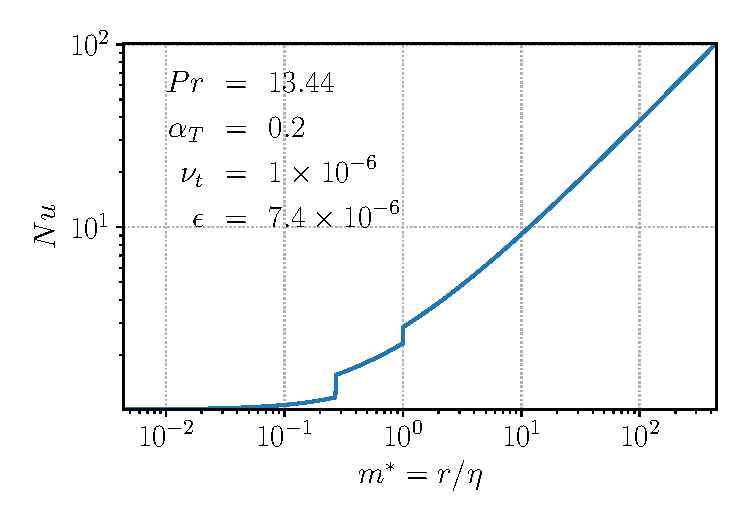
\includegraphics[width=0.65\textwidth]{graphics/figure_nusselt.pdf}
  \caption{Nusselt number as a function of the ratio $m^{*}$}
  \label{fig:nusselt}
\end{figure}
\end{enumerate}

\begin{WarningBlock}{Note:}
    When using \telkey{MODEL FOR THE NUSSELT NUMBER=2}, turbulent parameters need to be estimated using
    \telkey{MODEL FOR ESTIMATION OF TURBULENCE PARAMETERS=1 or 2}. See section \ref{turbulence} for additional details.
\end{WarningBlock}

%---------------------------------------------------------------------------
\subsection{Secondary nucleation}
\label{section:secondary_nucleation}

When frazil crystals collide, new nuclei are detached
which increases the volume fraction of the smallest particles.
This is known as the secondary nucleation process.
There are two variants of secondary nucleation model implemented in \khione
which can be selected with the keyword \telkey{MODEL FOR THE SECONDARY NUCLEATION} (default = 2):
\begin{lstlisting}
0 : NO SECONDARY NUCLEATION
1 : SVENSSON & OMSTEDT (1994)
2 : WANG & DOERING (2005)
\end{lstlisting}

Secondary nucleation is modeled  (in model 1 or 2) using an approximation of the
collision frequency between particles \cite{Omstedt_1994}.
A particle with a velocity $w^r_k$ relative to the fluid sweeps a volume $\delta V = w^r_k \pi r_k^2 \delta t$
during $\delta t$.
The collision frequency can be estimated as $f^k_{coll} \sim \widetilde{n} \delta V n_k / \delta t$,
in which $\widetilde{n}$ is an estimation of the average number of particles per unit volume, defined in Equation \eqref{eq:model:ssn:average_number_of_particle}
and $n_k$ the number of particles of class $k$ per unit volume.
\begin{equation}
\widetilde{n}=\max \left( \sum_{j=1}^{N_c} n_j, n_{max}\right).
\label{eq:model:ssn:average_number_of_particle}
\end{equation}
$n_{max}$ is a parameter used to limit collisions impact which
can be tuned using the \telkey{SECONDARY NUCLEATION NMAX PARAMETER} (default = 6.E6).
%A value of $n_{max}=10^3$ is suggested in \cite{Omstedt_1994}.
The relative velocity is estimated from the rising and turbulent velocities such that
\begin{equation}
w^r_k= \sqrt{ {U^t_k}^2+ w_k^2 },
\label{eq:model:ssn:relative_velocity}
\end{equation}
with
\begin{itemize}
	\item $U^t_k$ the turbulent velocity of crystals estimated by $U^t_k= 2 r_k \sqrt{ \frac{\epsilon}{15 \nu} }$,
	\item $w_k$ the buoyant rise velocity of frail crystals. Different models can be selected via the keyword \telkey{MODEL FOR THE BUOYANCY VELOCITY} (default = 1).
\end{itemize}
Finally, volume fraction change rate due to secondary nucleation can be written as:
\begin{equation}
S_{SN}^{k}=
\left\lbrace \begin{matrix}
\sum_{j=2}^{N} \pi \widetilde{n} w^r_j r_j^2 C_{j} & \text{if} & k=1 \\
-\pi \widetilde{n} w^r_k r_k^2 C_{k} & \text{if} & k \neq 1
\end{matrix} \right. .
\label{eq:model:ssn:source}
\end{equation}

Mass exchanges between classes due to the secondary nucleation process are schematized in Figure \ref{fig:secondary_nucleation}.

\begin{figure}[H]
    \begin{center}
        \includegraphicsmaybe{[width=0.45\textwidth]}{./graphics/secondary_nucleation.png}
    \end{center}
    \caption{Mass exchanges between classes due to secondary nucleation}
    \label{fig:secondary_nucleation}
\end{figure}

%---------------------------------------------------------------------------
\paragraph{Rise velocity of frazil crystals}
\label{buoyancy}
Different empirical approaches are proposed in the literature to estimate the rise velocity $w_k$.
The model can be selected via the keyword \telkey{MODEL FOR THE BUOYANCY VELOCITY} (default = 2):
\begin{lstlisting}
1 : DALY (1984)
2 : SVENSSON & OMSTEDT (1994)
3 : MATOUSEK (1992)
4 : GOSIK & OSTERKAMP (1983)
5 : MORSE & RICHARD (2009)
\end{lstlisting}

\begin{enumerate}
\item If \telkey{MODEL FOR THE BUOYANCY VELOCITY=1} the formulation proposed by Daly
\cite{daly_1984} for Stokes range,
intermediate range and fully turbulent range is used,
for which the rise velocity is given by:
\begin{equation}
w_k =
\left\lbrace
	\begin{matrix}
	& 0.08 ( g' r_k^2 / \nu ) \quad & \text{if} & \quad r_k \leq 3\cdot10^{-4} \\
  & 0.16 ( g'^{0.715} \nu^{-0.428} r_{k}^{1.14} ) \quad & \text{if} & \quad 3\cdot10^{-4} < r_k \leq 1.4\cdot10^{-3} \\
	& \sqrt{g' r_k/2} \quad & \text{if} & \quad r_k > 1.4 \cdot10^{-3},
\end{matrix}
\right.
\label{eq:model:rise_velocity_daly}
\end{equation}
in which
\begin{itemize}
    \item $g'= \dfrac{2 K_v g (\rho-\rho_i)}{\pi \rho}$ is the reduced gravitational acceleration,
	\item $K_v = 2 \pi /R$ is the volumetric shape factor.
\end{itemize}

\item Svensson and Omstedt \cite{Omstedt_1994} simplified the previous formulation into $w_k=32.8(2 r_k)^{1.2}$ which only takes into account the intermediate range (\telkey{MODEL FOR THE BUOYANCY VELOCITY=2}).

\item If \telkey{MODEL FOR THE BUOYANCY VELOCITY=3} an empirical formulation proposed by
Matousek \cite{matouvsek1992frazil} is used leading to:
\begin{equation}
w_k=1.31\cdot10^{-5}( 2 r_k^{0.29} e_k^{0.61} / \nu )
\end{equation}

\item If \telkey{MODEL FOR THE BUOYANCY VELOCITY=4} the formulation proposed by
Gosik and Osterkamp in \cite{gosink1983measurements} for fully turbulent range
is used and the rise velocity is estimated with:
\begin{equation}
w_k=\sqrt{\frac{4gr_k(\rho-\rho_i)}{R C_d \rho}}.
\label{eq:rise_velocity}
\end{equation}
in which $C_d$ is the drag coefficient.

\item If \telkey{MODEL FOR THE BUOYANCY VELOCITY=5} the formulation proposed by Morse and Richard
\cite{MORSE200986} is used, which reads (in mm-s units, with $d_k = 2 r_k$)
\begin{equation}
w_k =
\left\lbrace
	\begin{matrix}
	&  2.025 d_k^{1.621}               \quad & \text{if} & \quad d_k \leq 1.27 \text{ mm} \\
  & -0.103 d_k^2 + 4.069 d_k -2.024  \quad & \text{if} & \quad d_k > 1.27 \text{ mm} \\
\end{matrix}
\right.
\label{eq:model:rise_velocity_daly}
\end{equation}

\end{enumerate}

A review of rise velocity formulations is plotted on Figure \ref{fig:rise_velocity}.
\begin{figure}[H]
  \centering
  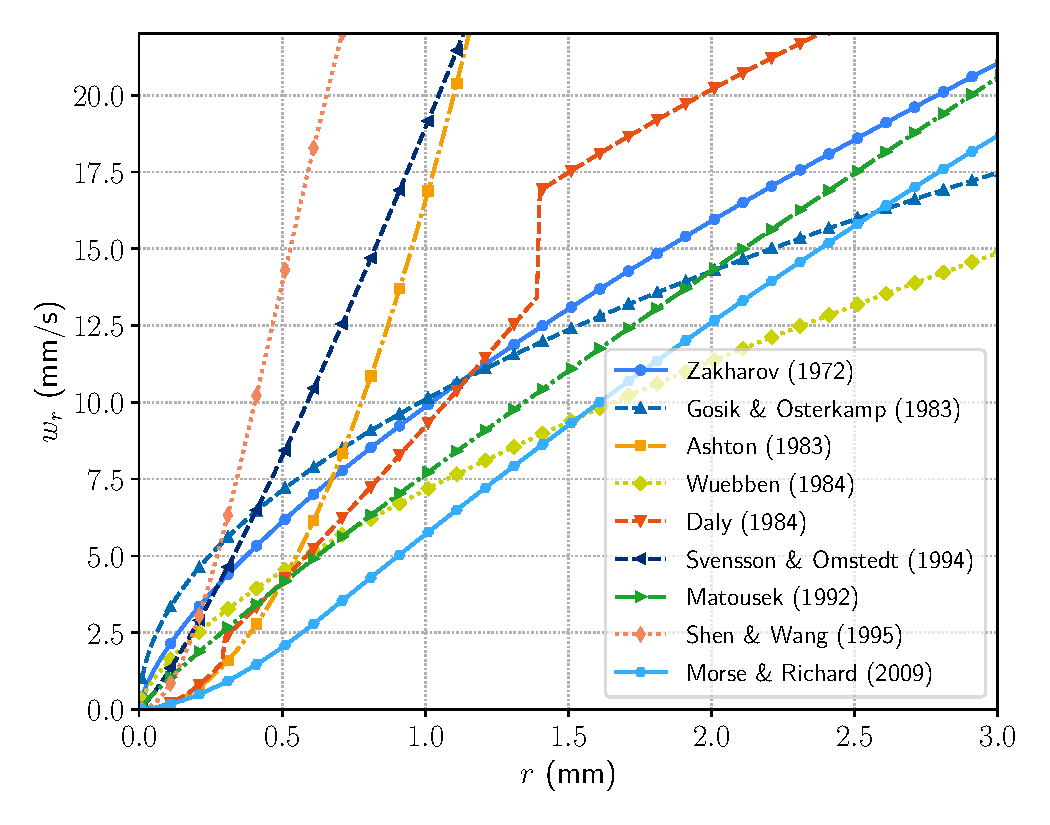
\includegraphics[width=0.65\textwidth]{graphics/figure_rise_velocity.pdf}
  \caption{Rise velocity formulations with $R=10$.}
  \label{fig:rise_velocity}
\end{figure}

%---------------------------------------------------------------------------
\subsection{Flocculation}
\label{section:flocculation}

The flocculation model can be selected with the keyword
\telkey{MODEL FOR THE FLOCCULATION AND BREAKUP} (default = 1):
\begin{lstlisting}
0 : NO FLOCCULATION
1 : SVENSSON AND OMSTEDT (1994)
\end{lstlisting}

If \telkey{MODEL FOR THE FLOCCULATION AND BREAKUP=1},
the flocculation source term is defined in Equation \eqref{eq:model:sfb:source} and schematized in
Figure \ref{fig:flocculation}.
\begin{equation}
S_{FB}^{k}=\beta_{k-1}C_{k-1} -\beta _{k}C_{k}.
\label{eq:model:sfb:source}
\end{equation}

\begin{figure}[H]
    \begin{center}
        \includegraphicsmaybe{[width=0.4\textwidth]}{./graphics/flocculation.png}
    \end{center}
    \caption{Mass exchanges between classes due to flocculation}
    \label{fig:flocculation}
\end{figure}

Floculation and breakup are supposed to result only in a net increase in scales \cite{Omstedt_1994}.
The effectiveness of class jumps is
supposed to be linearly dependent on radius:
\begin{equation}
\beta_k = a_{floc} \dfrac{r_k}{r_1},
\label{eq:model:sfb:beta_k}
\end{equation}
where
\begin{itemize}
	\item $a_{floc}$ represents the proportion of frazil crystals that move from class $k$ to $k+1$ per second,
    which can be tuned with the keyword \telkey{FLOCCULATION AFLOC PARAMETER} (default = 1.E3),
    \item $r_k$ is the radius of the $k^{\rm{th}}$ class,
    \item $r_1$ is the radius of the first class.
\end{itemize}



%---------------------------------------------------------------------------
\subsection{Seeding}
\label{section:seeding}

Modeling primary nucleation is still a major difficulty in frazil studies as the seeding process is
not fully understood yet. It depends on atmospheric conditions (snow, mist) and water impurities.
In \khione there are two ways to introduce primary nuclei in the media, which can be selected via the keyword
\telkey{MODEL FOR FRAZIL SEEDING} (default = 1):
\begin{lstlisting}
0 : NO SEEDING
1 : MINIMUM CONC. THRESHOLD
2 : CONSTANT SURFACIC SEEDING RATE
3 : BOTH OPTIONS 1 AND 2
\end{lstlisting}

\begin{enumerate}
\item If \telkey{MODEL FOR FRAZIL SEEDING=1} a minimum threshold of frazil volume fraction
is set to prevent frazil to decrease below this threshold. It is defined with a
minimum number of nuclei per unit volume, which can be tuned via the keyword
\telkey{MINIMUM NUMBER OF FRAZIL CRYSTALS} (default = 7.1586E4). If multiple classes are selected,
the number of primary nuclei is equally shared between all classes. Note that the default value was obtained from optimal calibration with Carstens experiments \cite{carstens_1966} alongside a default mean raidus of 4.1E-4 and a constant Nusselt number of 4. 

\item If \telkey{MODEL FOR FRAZIL SEEDING=2} a surfacic seeding rate is used, which corresponds
to a number of crystals reaching the water column through the free surface per second, noted $\tau_{seeding}$ in crystals.m$^{-2}$.s$^{-1}$.
The volumic seeding rate source term, which corresponds to the increase of the frazil volume fraction, noted $S^k_{SR}$ is then defined by $S^k_{SR} = V_k \times \tau_{seeding} /h$.
The surfacic seeding rate $\tau_{seeding}$ can be adjusted with the keyword
\telkey{FRAZIL SEEDING RATE} (default = 100.). An estimation of the seeding rate based on observations has been proposed in \cite{daly_1994} leading to a range of $3 \times 10^{-1}$ to $1$ crystals.cm$^{-2}$.s$^{-1}$.

\item Both methods of seeding can be selected by setting \telkey{MODEL FOR FRAZIL SEEDING=3}.
\end{enumerate}

\begin{WarningBlock}{Note:}
    If no seeding is selected i.e. \telkey{MODEL FOR FRAZIL SEEDING=0},
    the first melting event will cause a decrease of frazil volume fraction
    until it reaches $0$ making any further thermal growth of frazil impossible
    due to the nature of the model.
    Therefore the introduction of new nuclei with seeding methods 1, 2 or 3 are mandatory
    to allow multiple successive freeze-up and melting sequences.
\end{WarningBlock}

%---------------------------------------------------------------------------
\subsection{Deposition and erosion under the ice cover}
\label{section:precipitation}

Suspended frazil particles growing in size, may cluster
together, and move up to the water surface to either form surface ice, deposit on the bottom
of the ice cover, or attach on the bottom of ice pans. This upward movement is controlled by the
buoyancy velocity of the frazil ice particles and the strength of turbulence mixing. The ice flocs
on the water surface can also be entrained into the river flow when the turbulence intensity is
strong enough to overcome their buoyancy.
In the present model a sink term $S_M^k$ is introduced in Equation \ref{eq:model:frazil} to model mass transfer between suspended frazil ice and the ice cover.
Deposition and erosion can be activated with the keyword \telkey{MODEL FOR MASS EXCHANGE BETWEEN FRAZIL AND ICE COVER} (default = 0):
\begin{lstlisting}
0 : NO MASS EXCHANGE
1 : DEPOSITION ONLY
2 : DEPOSITION AND EROSION
\end{lstlisting}

Frazil ice particles rise to the surface at a rate which depends on concentration and on the rise velocity defined in Equation \ref{eq:rise_velocity}. 
The sink term for each class of frazil can be expressed as
\begin{equation}
S_M^k = -\dfrac{1}{h} \int_{z_b}^{\eta} \dfrac{ \partial w_k \overline{C_k}(z)}{ \partial z}  dz,
\end{equation}
in which
\begin{itemize}
	\item $z_b$ is the bottom elevation
	\item $\eta$ is the free surface elevation
	\item $\overline{C_k}(z)$ is the frazil volume fraction in the water column
\end{itemize}

To properly describe the net flux of frazil ice accumulating at the free surface, assumptions  
should be made on the vertical profile of frazil ice volume fraction and rise velocity but also on the physical deposition and erosion processes. \newline

\begin{enumerate}
\item 
If \telkey{MODEL FOR MASS EXCHANGE BETWEEN FRAZIL AND ICE COVER=1} only a net deposition flux is considered.
The source term $S_M^k$ is defined such that $S_M^k = -S_{MI}^k / h$ where $S_{MI}^k$ is defined is the section \ref{section:mass_exchanges}.
A constant volume fraction profile and a constant buoyant rise velocity are considered
leading to the following deposition/erosion source term: 
\begin{equation}
S_M^k= -\min \left( \dfrac{ D_k w_k C_k}{h} , \dfrac{C_k}{\Delta t} \right).
\end{equation}
in which
\begin{itemize}
	\item $w_k$ is the buoyancy velocity of class $k$ in m.s$^{-1}$, as defined in section \ref{buoyancy},
    \item $D_k$ is the probability of deposition of frazil particles reaching the surface for the class $k$ (between 0 and 1), which can be set via the keyword \telkey{FRAZIL UNDER COVER DEPOSITION PROBABILITY} (default = 1)
\end{itemize}

\item 
If \telkey{MODEL FOR MASS EXCHANGE BETWEEN FRAZIL AND ICE COVER=2} erosion and deposition are both considered. 
The source term $S_M^k$ is defined such that $S_M^k = -S_{MI}^k / h$ where $S_{MI}^k$ is defined is the section \ref{section:mass_exchanges}.
%The key parameters of the model are:
%\begin{itemize}
%    \item $D_k$ is the probability of deposition of frazil particles reaching the surface for the class $k$ (between 0 and 1), which can be set via the keyword \telkey{FRAZIL UNDER COVER DEPOSITION PROBABILITY} (default = 1)
%  \item $E_k$ is the coefficient of re-entrainment rate of surface ice per unit area in s$^{-1}$ for the class $k$, which can be set via the keyword \telkey{FRAZIL UNDER COVER REENTRAINMENT COEFFICIENT} (default = 1.E-4).
%\end{itemize}

\end{enumerate}

\begin{WarningBlock}{Note:}
In addition to frazil conservation equations, a mass balance equation for the surface ice layer needs to be introduced to ensure total ice mass conservation. This can be achieved by introducing a dynamic ice cover model 
with the keyword \telkey{DYNAMIC ICE COVER} = YES (default=NO) as described in section \ref{section:dynamics_ice_cover}.
\end{WarningBlock}

%---------------------------------------------------------------------------
\section{Thermal balance}
\label{thermal_balance}

The water fraction of the water-ice mixture is characterized
by a temperature, subject to a heat balance defined as:
\begin{equation}
\frac{\partial }{\partial t} \left[ (1-C)T \right]  + \nabla. \left[ (1-C) \vec{u} T \right]  = \dfrac{1}{h}  \nabla .(h \nu_{t,T} \nabla \left[ (1-C) T \right] ) +\frac{\phi_s }{h \rho c_{p}} - \frac{1}{\rho c_{p}}( S_{L} + S^{ic}_L)
\label{eq:model:temperature_water_phase}
\end{equation}
where
\begin{itemize}
	\item $c_{p}= 4.1855 \times 10^3$ J.kg$^{-1}$.K$^{-1}$ is the specific heat of water,
	\item $\phi_s$ is the net heat flux at the free surface in W.m$^{-2}$,
	\item $S_{L}$ is the heat source due to melting or freezing of frazil ice expressed in W.m$^{-3}$,
	\item $S^{ic}_{L}$ is the heat source due to melting or freezing of the ice cover in W.m$^{-3}$, defined in section \ref{section:thermal_growth_icover}.
\end{itemize}

The net heat flux at free surface $\phi_s$ is equal to $\phi_{aw}$ in absence of ice cover.
If ice cover is present, the net heat flux received by water is combination of the fraction of
the heat flux coming from the atmosphere to the water surface and the heat exchange with the ice cover layer,
therefore $\phi_s$ can be expressed as:
\begin{equation}\label{heat_fluxes_water}
\phi_s = (1-C_i) \phi_{aw} + C_i (\phi_{iw} + \phi_{ai}),
\end{equation}
in which
\begin{itemize}
	\item $C_i$ is the surface ice fraction (portion of free surface covered by ice),
	\item $\phi_{iw}$ is the convective heat flux between the surface ice layer and the water column.
\end{itemize}
The heat source due to melting or freezing can be expressed as:
\begin{equation}
S_{L}= \rho L_i \delta_w - \rho c_p T_i \delta_w,
\end{equation}
where
\begin{itemize}
	\item $T_i$ the crystal temperature, assumed to be equal to the freezing temperature,
	\item $\delta_w$ is the water volume change rate (s$^{-1}$) due to frazil ice evolution,  expressed as
\end{itemize}
\begin{equation}
\delta_w = - \frac{\rho_i}{\rho} \sum_{k=1}^{N_c} S^k_{GM}.
\label{eq:dw}
\end{equation}

For simplicity's sake, let us neglect $S_L^{ic}$, Equation \eqref{eq:model:temperature_water_phase} can be developed as:
\begin{equation}
(1-C)\frac{\partial T}{\partial t}+(1-C) \vec{u}. \nabla T =
\dfrac{1}{h}  (1-C) \nabla .(h \nu_{t,T} \nabla T)-2 \nu_{t,T} \nabla T. \nabla C+\frac{\phi_s }{h \rho c_{p}}
- \delta_w \left( T - T_f + \frac{L_i}{ c_{p}} \right).
\label{eq:model:temperature_water_phase_developped}
\end{equation}
Additionally, the term $2 \nu_{t} \nabla T. \nabla C$ in Equation \eqref{eq:model:temperature_water_phase_developped} can be neglected after \cite{holland_JFM_2005}, considering the hypothesis that $C\ll1$.
Hence, the heat balance Equation \eqref{eq:model:temperature_v1} is obtained.
\begin{equation}
\frac{\partial T}{\partial t} + \vec{u}. \nabla T= \dfrac{1}{h} 
\nabla .(h \nu_{t,T} \nabla T)
+\frac{\phi_s }{h \rho c_{p} (1-C)}
+ \frac{ \rho_i}{ \rho (1-C)}
\left(T - T_f + \frac{L_i}{ c_{p}} \right) \sum_{k=1}^{N_c} S^k_{GM}.
\label{eq:model:temperature_v1}
\end{equation}
Equation \eqref{eq:model:temperature_v1} can be further simplified by considering $C\ll1$ and $T-Tf \ll \frac{L_i}{c_p}$, which leads to:
\begin{equation}
\frac{\partial T}{\partial t}+ \vec{u}. \nabla T= \dfrac{1}{h} \nabla .( h\nu_{t,T} \nabla T) + \frac{\phi_s }{h \rho c_{p}}
+\frac{\rho_i L_i}{\rho c_{p}} \sum_{k=1}^{N_c} S^k_{GM}.
\label{eq:model:temperature_v2}
\end{equation}
Both Equations \eqref{eq:model:temperature_v1} and \eqref{eq:model:temperature_v2} are implemented
in \khione and can be selected via the keyword \telkey{ENERGY BALANCE VERSION} (default = 1):
\begin{lstlisting}
1 : SIMPLIFIED ENERGY BALANCE
2 : FULL ENERGY BALANCE
\end{lstlisting}

For the SSC frazil ice model (when only one class of frazil is selected),
Equations \eqref{eq:model:temperature_v1} and \eqref{eq:model:temperature_v2} still
hold by replacing $\sum_{k=1}^{N_c} S^k_{GM}$ by $S_{GM}$.
Note that $S_L^{ic}$ is taken into account in both formulations in presence of an ice cover.

%---------------------------------------------------------------------------
\section{Salinity balance}
\label{salinity_balance}

The salinity can be activated in the model with the keyword \telkey{SALINITY} (default = NO).
If  \telkey{SALINITY=YES}, the salinity balance is given by:
\begin{equation}
\frac{\partial S}{\partial t} + \vec{u}. \nabla S = \dfrac{1}{h}  \nabla . \left( h \nu_{t,S} \nabla S \right)
+ S_{R} ,
\label{eq:model:salinity}
\end{equation}
in which
\begin{itemize}
	\item $\nu_{t,S}$ is the turbulent diffusivity,
	\item $S_{R}$ is the salt rejection source term caused by the freezing or melting of frazil ice.
\end{itemize}
Salt rejection can be expressed as a function of the water phase rate of volume change $\delta_w$.
The salinity rejection source can be calculated as in Equation \eqref{eq:model:salinity_rejection}
\begin{equation}
S_{R} = \frac{\rho_i}{\rho} (S-S_i) \sum_{k=1}^{N_c} S^k_{GM},
\label{eq:model:salinity_rejection}
\end{equation}
with
\begin{itemize}
	\item $S_i$ the salinity of frazil crystals assumed to be equal to zero.
\end{itemize}

For the SSC frazil ice model (when only one class of frazil is selected),
Equation \eqref{eq:model:salinity_rejection} still
holds by replacing $\sum_{k=1}^{N_c} S^k_{GM}$ by $S_{GM}$.

%---------------------------------------------------------------------------
\section{Turbulence}
\label{turbulence}

Turbulence parameters required to compute the different sources defined above
can be estimated via different approaches selected via the keyword
\telkey{MODEL FOR ESTIMATION OF TURBULENCE PARAMETERS} (default = 1):
\begin{lstlisting}
0 : CONSTANT VALUES
1 : MIXING LENGTH MODEL, SHEN (2010)
2 : K-EPS MODEL OF TELEMAC-2D
\end{lstlisting}

\begin{enumerate}
\item If \telkey{MODEL FOR ESTIMATION OF TURBULENCE PARAMETERS=0}, 
the turbulent kinetic energy $k$, the turbulent kinetic energy dissipation rate $\epsilon$
 and the turbulent intensity $\alpha_{T}$ need 
to be provided with the keyword
\telkey{CONSTANT TURBULENCE PARAMETERS}
 (default: $9.6 \times 10^{-4}$;$12 \times 10^{-4}$;$8.7 \times 10^{-2}$).
These constant parameters will only affect the computation of the Nusselt number
 (cf. section \ref{paragraph:nusselt}).
\item If \telkey{MODEL FOR ESTIMATION OF TURBULENCE PARAMETERS=1}, the model
suggested in \cite{shen_JHR_2010} is used which
relies on a depth averaged integration of $k$ and $\epsilon$
profiles defined as in Equations \eqref{eq:model:k_profile} and \eqref{eq:model:eps_profile}.
\begin{equation}
k(z)=\frac{u_{*}^{2}}{\sqrt{C_{\mu}}}(1-\frac{z}{h}),
\label{eq:model:k_profile}
\end{equation}
\begin{equation}
\epsilon (z)=\frac{u_{*}^{3}}{\kappa z }(1-\frac{z}{h}),
\label{eq:model:eps_profile}
\end{equation}
in which $u_{*}$ is the friction velocity.
The profiles are integrated between the upper bound of the
viscous boundary layer and the free surface \cite{shen_JHR_2010}.
\item If \telkey{MODEL FOR ESTIMATION OF TURBULENCE PARAMETERS=2} turbulence parameters
are estimated using the $k$-$\epsilon$ solver from \telemac{2D}.
\end{enumerate}

Turbulent viscosities are then computed as $\nu_{t} = C_{\mu} \frac{k^2}{\epsilon}$.

%---------------------------------------------------------------------------
\section{Clogging or frazil accretion on racks}
\label{chapter:clogging}

Frazil accretion on racks can occur when the water temperature is supercooled. While there is no analytical formulation available, a few laboratory and field studies have been published on the topic (\cite{daly1991frazil}, \cite{andersson1992frazil}, \cite{andersson1992laboratory} and \cite{richard2008multiple}).\newline

The growth of ice on the rack is predominately due to the deposition of suspended frazil on the rack bars (\cite{daly1987modeling}). The Figure \ref{fig:vertical_clogging} shows the typical processes of frazil accretion on the trash rack bars (\cite{daly1991frazil}).\newline

\khione allows the accretion of ice on either one set of bars (vertical or horizontal) or a combined mesh (vertical and horizontal), the difference being based on the geometry of frazil accretion and blockage. It is important to note that the retro-action of the accumulated ice on the flow is not taken into account.\newline

\begin{figure}[H]
    \begin{center}
        \includegraphicsmaybe{[scale=0.4]}{./graphics/clogging_1.png}
    \end{center}
    \caption{Stages of frazil accretion on a rack of vertical bars}
    \label{fig:vertical_clogging}
\end{figure}

\subsection{Inputs and outputs}

This physical process can be activated with the keyword \telkey{CLOGGING ON BARS} = YES (default is NO).\newline

It is possible to activate this process on a liquid boundary, by specifying its number with the keyword \telkey{CLOGGED BOUNDARY NUMBERS} (default = 0). If several boundary numbers are given, the clogging process appends on all of them.\newline

It is also possible to simulate the clogging on sections in the middle of the computational domain. The keyword \telkey{CLOGGED SECTIONS} must then be given, with the nodes corresponding to the section extremity. For example, if one wants to compute the clogging on two sections, the first between nodes 125 and 256 and the second between nodes 267 and 52, the steering file should contain the keyword \telkey{CLOGGED SECTIONS} = 125;256 ; 267;52.\newline

The results of the clogging are saved in the file with the name specified with the keyword \telkey{CLOGGING RESULTS FILE}. It contains the accumulated mass and volume of ice on the rack and the available area for the water in an ASCII file for all the clogged sections and boundaries.\newline

\subsection{Clogging on a set of vertical or horizontal bars}

The physical properties of the bars are set through the keyword \telkey{PHYSICAL CHARACTERISTICS OF THE INTAKE RACK}. The dimension of this keyword is 4. The default value is 0.06; 0.01; 0.06; 0.01. The values represent:

\begin{enumerate}
 \item distance between the centre of the transverse bars,
 \item diameter of the transverse bars,
 \item distance between the centre of the vertical bars,
 \item diameter of the vertical bars.
\end{enumerate}

To consider only vertical bars, the diameter of horizontal bars must be set to zero and vice versa. In the following, the diameter of the bars set with this keyword corresponds to the variable $l_B$, and the distance between the bars is used to compute $n_B$ the number of bars in the section.

It is estimated from Figure \ref{fig:vertical_clogging} that the angle $\alpha$ between the edge of frazil accumulation and the transverse direction is $55^{\circ}$. The width of the gap between two bars with ice accumulation is $d_w$. Since the flow passes through the submerged rack, it is assumed that the frazil ice is uniformly distributed over its cross-section. This assumption could be removed at a later stage.\newline

\begin{figure}[H]
    \begin{center}
        \includegraphicsmaybe{[scale=0.4]}{./graphics/clogging_2.png}
    \end{center}
    \caption{Geometry of frazil accretion on a bar}
    \label{fig:bar_clogging}
\end{figure}

The frazil deposition is assumed to start from the front face of the bars, as shown in the blue colored arch within the angle $2\theta$ in Figure \ref{fig:bar_clogging} above, where $\theta$ is about $35^{\circ}= 90^{\circ}-55^{\circ}$ by default. The keyword \telkey{ANGLE OF ACCUMULATED ICE} (default = 35) allows to modify the value of $\theta$. The deposition efficiency of the frazil is assumed to be 1.0 to be conservative. \newline

The volume of frazil ice accumulation on a bar can be expressed as

\begin{equation} \label{eq:vol_frice_acc}
\nabla = \big[\theta r^2 - ({r_0}^2\sin\theta \cos\theta + 2\theta r_B^2 - r_B^2 \sin 2\theta \cos 2\theta)\big]l_B
\end{equation}

in which,
\begin{itemize}
    \item $\nabla$ is the volume of frazil ice accumulation,
    \item $r$ is the radius of the frazil ice accumulation,
    \item $r_0$ is the initial radius before the frazil ice accumulation, and
    \item $l_B$ is the length of the bar.
\end{itemize}

The volumetric rate of frazil ice accumulation can be written as

\begin{equation} \label{eq:vol_frice_rate1}
\dfrac{d\nabla}{dt} = 2\theta rl_B \frac{dr}{dt}
\end{equation}

or

\begin{equation} \label{eq:vol_frice_rate2}
  \dfrac{d\nabla}{dt} = \dfrac{q_{cv}w_f \alpha_f}{1-e_f}
\end{equation}

in which,
\begin{itemize}
    \item $q_{cv} = V_fHC_v$ is the unit width discharge of frazil ice volume,
    \item $V_f$ is the frazil velocity, assumed to be equal to water velocity normal to the grid,
    \item $C_v$ is volumetric frazil ice concentration,
    \item $w_f=2r\sin\theta$ is the frontal width for the frazil ice accumulation,
    \item $\alpha_f$ is the deposition coefficient, 1.0, and
    \item $e_f$ is the porosity, set to 0.67 by default after \cite{andersson1992laboratory}. This value can be modified through the keyword \telkey{POROSITY OF ACCUMULATED ICE}.
\end{itemize}

Equations \eqref{eq:vol_frice_rate1} and \eqref{eq:vol_frice_rate2} give

\begin{equation} \label{eq:front_frice_rate1}\dfrac{dr}{dt} = \dfrac{q_{cv}}{\theta l_B(1-e_f)}\sin\theta \alpha_f
\end{equation}

and

\begin{equation} \label{eq:front_frice_rate2}
\dfrac{dw_f}{dt} = \dfrac{q_{cv}}{\theta l_B(1-e_f)}2{\sin}^2\theta \alpha_f
\end{equation}

Equation \eqref{eq:front_frice_rate2} determines the growth rate of the frontal width of the frazil ice accumulation. Its finite difference form is

\begin{equation} \label{eq:front_frice_rate3}
{w_f}^{i+1} = {w_f}^i +\Delta t \dfrac{q_{cv}}{\theta l_B(1-e_f)}2{\sin}^2\theta \alpha_f
\end{equation}

The flow passage through the openings between two bars can be calculated:

\begin{equation} \label{eq:flow_passage}
d_w = d-w_f
\end{equation}

in which,
\begin{itemize}
    \item $d$ is centre to centre distance between two bars, and
    \item $d_w$ is the width of the available flow passage.
\end{itemize}


\subsection{Clogging on a grid of vertical and horizontal bars}

The calculations of the frazil clogging on the vertical and transverse bars follow the same procedures. Therefore, the available flow area for one grid can be calculated as

\begin{equation} \label{eq:avail_flow_area}
A_w = D_{w,V}l_{B,V}(n_V-1)-w_{f,T}\big[l_{B,T}-n_Vmax(d_{B,V},w_{f,T})\big]n_T
\end{equation}

in which,
\begin{itemize}
    \item subscripts $V$ and $T$ represent the vertical and transverse bars,
    \item $n_B$ is number of bars, and
    \item $l_B$ is the length of the bar
\end{itemize}


\renewcommand{\labelitemi}{\textbullet}

\clearpage
